\documentclass[11pt,a4paper]{article}

% Language setup for Greek and English
\usepackage[english,greek]{babel}
\usepackage[utf8]{inputenc}
\usepackage[T1,LGR]{fontenc}

% Fonts (matches the user template style)
\usepackage{fontspec}
\setmainfont{Linux Libertine O}[Scale=0.95]
\setsansfont{Linux Biolinum}[Scale=0.95]
\setmonofont{DejaVu Sans Mono}[Scale=0.85]

% Layout
\usepackage[a4paper,top=2.2cm,bottom=2.2cm,left=2.4cm,right=2.4cm]{geometry}
\usepackage{parskip}
\setlength{\parindent}{0pt}
\setlength{\parskip}{4pt}

% Tables and figures
\usepackage{graphicx}
\usepackage{booktabs}
\usepackage{array}
\usepackage{amsmath}
\usepackage{caption}
\captionsetup{font=small,labelfont=bf}

% TikZ for the architecture diagram
\usepackage{tikz}
\usetikzlibrary{positioning, arrows.meta, shapes.geometric, fit, backgrounds}

% Colors and links
\usepackage{xcolor}
\definecolor{linkBlue}{HTML}{1976D2}
\usepackage{hyperref}
\hypersetup{
   colorlinks=true,
   linkcolor=linkBlue,
   citecolor=linkBlue,
   urlcolor=linkBlue,
   unicode=true,
   pdftitle={Επεξεργασία Δεδομένων Ροής με Kafka, Spark και MongoDB},
   pdfsubject={Αναφορά Project, CEID\_NE4348, 2026}
}

% Bibliography
\usepackage[numbers,square,sort\&compress]{natbib}
\bibliographystyle{hellas}

% Compact section titles
\usepackage{titlesec}
\titleformat{\section}{\large\bfseries}{\thesection.}{0.5em}{}
\titleformat{\subsection}{\normalsize\bfseries}{\thesubsection}{0.5em}{}
\titlespacing*{\section}{0pt}{8pt}{2pt}
\titlespacing*{\subsection}{0pt}{4pt}{1pt}

% Code-like inline
\newcommand{\code}[1]{\texttt{\small #1}}

\begin{document}

% ====================== Title block ======================
\begin{center}
   {\Large\bfseries Επεξεργασία Δεδομένων Ροής με Kafka, Spark και MongoDB}\\[4pt]
   {\small Project Εαρινού Εξαμήνου 2026 \textbar{} Συστήματα Διαχείρισης Μεγάλων Δεδομένων}\\[2pt]
   {\small Τμήμα Μηχανικών Η/Υ και Πληροφορικής, Πανεπιστήμιο Πατρών}\\[2pt]
   {\small Βασίλειος Μπίτζας \textbar{} Μάιος 2026}
\end{center}
\vspace{3pt}\hrule\vspace{6pt}

% ====================== §1 Introduction ======================
\section{Εισαγωγή}
Η εργασία υλοποιεί ένα ολοκληρωμένο pipeline ανάλυσης ροής δεδομένων κυκλοφορίας. Δεδομένα οχημάτων που παράγονται από τον προσομοιωτή UXSIM αποστέλλονται σε έναν Kafka-συμβατό broker (Redpanda), καταναλώνονται σε πραγματικό χρόνο από Spark Structured Streaming και αποθηκεύονται τόσο σε ακατέργαστη όσο και σε συγκεντρωτική μορφή σε MongoDB. Όλη η στοίβα τρέχει τοπικά μέσω Docker Compose με μία εντολή (\code{docker compose up -d}) για τα 6 βασικά services, ή με ενεργοποίηση όλων των profiles ώστε να σηκωθούν επιπλέον το REST API και το dashboard: \newline\code{docker compose --profile api --profile dashboard up -d}

Η παρούσα αναφορά καλύπτει τα τρία ζητούμενα ερωτήματα της εκφώνησης (παραγωγή προς Redpanda, επεξεργασία με Spark, αποθήκευση σε MongoDB) και επιπλέον τρία bonus που υλοποιήθηκαν: (i) windowed aggregations 30 δευτερολέπτων με min/max ταχύτητα ανά link, (ii) REST API με FastAPI πάνω από τη MongoDB και (iii) Streamlit dashboard με ζωντανό χάρτη δικτύου σε Plotly. Για περισσότερα σχετικά με το project, μπορείτε να επισκεφθείτε το repository στο \href{https://github.com/IBilba/traffic-streaming-pipeline}{traffic-streaming-pipeline}.

% ====================== §2 Architecture ======================
\section{Αρχιτεκτονική Συστήματος}

\begin{figure}[!h]
\centering
% Layout follows traffic_streaming_pipeline_dataflow.svg; box fills use the
% pastel category palette (broker/compute/store/ui) instead of the SVG dark theme.
\definecolor{dfTitle}{HTML}{151515}
\definecolor{dfArrGray}{HTML}{94A3B8}
\definecolor{dfArrBlue}{HTML}{2563EB}
\definecolor{dfArrOrange}{HTML}{D97706}
% The SVG viewBox is 0 0 1000 620 with y growing downward; we reuse those raw
% coordinates and flip y (y is negative) so the layout matches the SVG exactly.
\begin{tikzpicture}[
   x=0.0145cm, y=-0.0145cm,
   bx/.style={draw=black, line width=0.5pt, rounded corners=4pt},
   broker/.style={bx, fill=blue!8},
   compute/.style={bx, fill=orange!10},
   store/.style={bx, fill=green!10},
   ui/.style={bx, fill=violet!10},
   lbl/.style={anchor=base, inner sep=0pt, outer sep=0pt},
   ttl/.style={lbl, text=black, font=\scriptsize\bfseries},
   sub/.style={lbl, text=black!55, font=\tiny},
   subm/.style={sub, font=\tiny\ttfamily},
   arr/.style={-{Stealth[length=1.6mm]}, line width=0.55pt},
   arg/.style={arr, draw=dfArrGray},
   arbl/.style={arr, draw=dfArrBlue},
   aror/.style={arr, draw=dfArrOrange}
]
% ---- Boxes ----
% Spark cluster is shifted right (+56) and the MongoDB column further right
% (+120) versus the SVG so the "read" and "foreachBatch" arrow labels get
% open horizontal gaps instead of sitting on top of the boxes.
\draw[bx] (20,250) rectangle (192,382);      % producer
\draw[broker] (232,272) rectangle (350,364);     % redpanda
\draw[compute] (400,158) rectangle (652,450); % spark cluster
\draw[bx, fill=white] (418,200) rectangle (634,262);     % spark-master
\draw[bx, fill=white] (418,276) rectangle (634,338);     % spark-worker
\draw[bx, fill=white] (418,352) rectangle (634,426);     % spark-job
\draw[store] (842,150) rectangle (1042,212);    % raw_data
\draw[store] (842,300) rectangle (1042,362);    % stats
\draw[store] (842,450) rectangle (1042,512);    % stats_windowed
\draw[ui] (400,548) rectangle (1042,604);    % serving

% ---- Title ----
\node[lbl, text=dfTitle, font=\small\bfseries] at (531,32) {Traffic Streaming Pipeline: ροή δεδομένων};

% ---- Producer ----
\node[ttl]  at (106,278) {uxsim-producer};
\node[subm] at (106,302) {build\_grid\_network()};
\node[subm] at (106,322) {simulate\_traffic()};
\node[subm] at (106,342) {kafka\_publisher};
\node[sub]  at (106,366) {προσομοίωση → JSON};

% ---- Redpanda ----
\node[ttl]  at (291,302) {Redpanda};
\node[sub]  at (291,322) {Kafka-API broker};
\node[subm] at (291,344) {topic: uxsim};

% ---- Spark cluster ----
\node[ttl]  at (526,184) {Spark Structured Streaming};
\node[ttl]  at (526,224) {spark-master};
\node[sub]  at (526,244) {συντονιστής cluster};
\node[ttl]  at (526,300) {spark-worker};
\node[sub]  at (526,320) {executors (CPU/RAM, tasks)};
\node[ttl]  at (526,376) {spark-job = driver};
\node[subm] at (526,396) {run\_consumer.py};
\node[sub]  at (526,414) {readStream → parse → agg};

% ---- MongoDB collections ----
\node[lbl, text=black!60, font=\scriptsize\bfseries] at (942,132) {MongoDB · βάση: traffic};
\node[ttl]  at (942,176) {raw\_data};
\node[sub]  at (942,196) {ωμά events (verbatim)};
\node[ttl, font=\scriptsize\bfseries\ttfamily] at (942,326) {stats};
\node[sub]  at (942,346) {σύνοψη ανά (t, link)};
\node[ttl, font=\scriptsize\bfseries\ttfamily] at (942,476) {stats\_windowed};
\node[sub]  at (942,496) {παράθυρα 30s};

% ---- Serving ----
\node[ttl]  at (721,572) {FastAPI API \ + \ Streamlit dashboard};
\node[subm] at (721,590) {repository.py · evaluation/* (read-only queries)};

% ---- Arrows: producer -> redpanda -> spark ----
\draw[arg] (192,316) -- (232,316);
\node[sub] at (212,309) {JSON};
\draw[arg] (350,316) -- (400,316);
\node[sub] at (375,309) {read};

% ---- Fan-out trunk from spark to mongo ----
\draw[arg] (652,400) -- (775,400);
\node[subm] at (713,392) {foreachBatch};
\draw[draw=dfArrGray, line width=0.55pt] (775,181) -- (775,481);

% ---- raw branch (append) ----
\draw[arbl] (775,181) -- (842,181);
\node[lbl, text=dfArrBlue, font=\tiny\bfseries] at (808,173) {append};
% ---- stats branch (update) ----
\draw[aror] (775,331) -- (842,331);
\node[lbl, text=dfArrOrange, font=\tiny\bfseries] at (808,323) {update};
% ---- windowed branch (append) ----
\draw[arbl] (775,481) -- (842,481);
\node[lbl, text=dfArrBlue, font=\tiny\bfseries] at (808,473) {append};

% ---- mongo -> serving ----
\draw[arg] (942,512) -- (942,548);
\node[sub] at (970,534) {read};
\end{tikzpicture}
\caption{Ροή δεδομένων από τον προσομοιωτή ως την παρουσίαση. Όλα τα κουτιά είναι ανεξάρτητα containers στο ίδιο bridge network (\code{dsnet}).}
\label{fig:arch}
\end{figure}

Η στοίβα αποτελείται από έξι default containers και δύο προαιρετικά πίσω από Docker Compose profiles (Πίνακας~\ref{tab:containers}). Όλες οι υπηρεσίες επικοινωνούν μέσω του εσωτερικού bridge δικτύου \code{dsnet} και αναζητούνται με DNS βάσει του service name (π.χ.\ \code{redpanda:9092}, \code{mongo:27017}). Ο Redpanda εκθέτει επιπλέον έναν εξωτερικό listener στο \code{localhost:19092} για host-side εργαλεία (\code{rpk}, Compass). Η MongoDB είναι mapped στο \code{27018:27017} στον host ώστε να μη συγκρούεται με τυχόν τοπική εγκατάσταση MongoDB.

\begin{table}[h]
\centering\small
\begin{tabular}{@{}lll@{}}
\toprule
\textbf{Service} & \textbf{Ρόλος} & \textbf{Ports (host)} \\
\midrule
\code{redpanda}        & Kafka-API broker (single node)                & 9092, 19092, 9644 \\
\code{topic-init}      & One-shot job: δημιουργεί topic \code{UXSIM}   & --- \\
\code{UXSIM-producer}  & UXSIM simulation + Kafka publisher            & --- \\
\code{spark-master}    & Spark standalone master                       & 7077, 8080 \\
\code{spark-worker}    & Spark worker                                  & 8081 \\
\code{spark-job}       & Driver που τρέχει το consumer                 & 4040 \\
\code{mongo}           & MongoDB Community 7.0                         & 27018 \\
\code{traffic-api}     & FastAPI REST (\code{--profile api})           & 8000 \\
\code{dashboard}       & Streamlit + Plotly (\code{--profile dashboard}) & 8501 \\
\bottomrule
\end{tabular}
\caption{Υπηρεσίες του \code{docker-compose.yml}.}
\label{tab:containers}
\end{table}

\textbf{Δικαιολόγηση επιλογών.} Επιλέχθηκε ο Redpanda αντί για κλασική εγκατάσταση Kafka γιατί είναι μονό binary χωρίς JVM/ZooKeeper, μειώνοντας τους πόρους και τον χρόνο εκκίνησης ενώ διατηρεί πλήρη συμβατότητα στο wire protocol. Για το streaming layer προτιμήθηκε το Spark Structured Streaming αντί για το παλαιότερο Spark Streaming/DStreams, καθώς προσφέρει δηλωτικό DataFrame API και exactly-once σημασιολογία στους sinks. Η MongoDB διαλέχθηκε ως document store γιατί το payload του UXSIM είναι ήδη ημι-δομημένο JSON και δεν απαιτεί ρητό σχήμα στη βάση.

% ====================== §3 Design ======================
\section{Σχεδιαστικές Αποφάσεις}

\textbf{Functional core, OOP shell.} Όλα τα aggregations είναι καθαρές συναρτήσεις \code{DataFrame $\rightarrow$ DataFrame} χωρίς πλευρενέργειες (\code{compute\_link\_stats}, \code{compute\_windowed\_stats}). Στιγμιότυπα κλάσεων χρησιμοποιούνται μόνο όπου υπάρχει πραγματικός κύκλος ζωής: \code{KafkaProducer}, \code{SparkSession}, \code{TrafficRepository}. Όλη η είσοδος/έξοδος (Kafka read, Mongo write, REST handlers) ζει στις άκρες (\code{scripts/}, \code{ingestion/}, \code{serving/}).

\textbf{Output mode ανά sink.} Η επιλογή \code{outputMode} έγινε χωριστά για κάθε query: το \code{raw\_data} sink χρησιμοποιεί \code{append} (δεν υπάρχει ομαδοποίηση)· το \code{stats} sink χρησιμοποιεί \code{update} επειδή το \code{groupBy(t, link)} είναι αόριστο στο χρόνο και δε θέλουμε late-event drops· το \code{stats\_windowed} sink χρησιμοποιεί \code{append} με \code{withWatermark("t", "60 seconds")} ώστε να εκπέμπει closed windows. Κάθε query έχει τον δικό του φάκελο checkpoint, όπως απαιτεί ο Spark.

\textbf{Configuration layering.} Οι παράμετροι ακολουθούν αυστηρά την προτεραιότητα YAML (\code{config/default.yaml}) $<$ environment variables $<$ CLI flags. Στο Spark container το YAML είναι μη διαθέσιμο, οπότε τα env vars είναι η authoritative πηγή εκεί. Τίποτα δεν είναι hard-coded μέσα στον κώδικα (broker addresses, topic name, collection names, simulation seed).

\textbf{Πλήρης γραμμή στο schema.} Ο UXSIM εκθέτει status rows με \code{link} ίσο με \code{waiting\_at\_origin\_node} ή \code{trip\_end}. Διατηρούνται ως έχουν στον parser και φιλτράρονται \emph{μέσα} στη συνάρτηση aggregation με παράμετρο, ώστε τα tests να μπορούν να την καλέσουν με κενό σύνολο φίλτρων χωρίς duplication.

\textbf{Σημείο προσοχής στη γλώσσα του πεδίου.} Η εκφώνηση αναφέρεται στις στήλες ως \code{speed} και \code{time}. Ο UXSIM εκθέτει στην πραγματικότητα \code{v} (km/h) και \code{t} (seconds since simulation start). Η σύμβαση που ακολουθήθηκε είναι να αλιεύεται η αυθεντική στήλη του simulator και το rename σε \code{vspeed}/\code{vcount} να γίνεται μόνο στο επίπεδο του aggregation, ώστε να συμπίπτει με τους όρους της εκφώνησης στο τελικό sink.

% ====================== §4 Implementation per question ======================
\section{Υλοποίηση ανά Ερώτημα}

\subsection{Ερώτημα 1: UXSIM $\rightarrow$ Redpanda}
Το \code{ingestion/traffic\_simulator.py} τρέχει έναν δομημένο 4$\times$4 κόμβο road network (\code{ingestion/UXSIM\_network.py}), προχωράει την προσομοίωση ανά step και καλεί την \code{World.analyzer.vehicles\_to\_pandas()} για να πάρει το τρέχον στιγμιότυπο οχημάτων. Το \code{ingestion/kafka\_publisher.py} σειριοποιεί κάθε γραμμή ως JSON και δημοσιεύει στο topic \code{UXSIM}, με exponential backoff σε αποτυχίες σύνδεσης. Η παράμετρος \code{PRODUCE\_INTERVAL\_SEC} καθορίζει το wall-clock βήμα μεταξύ δύο simulation steps. Το topic δημιουργείται αυτόματα από το one-shot service \code{topic-init}, ο producer εξαρτάται μέσω \code{depends\_on: service\_completed\_successfully} ώστε να εξαλείφεται το race condition του πρώτου boot.

\subsection{Ερώτημα 2: Spark Structured Streaming consumer}
Το \code{preprocessing/schemas.py} ορίζει το \code{UXSIM\_EVENT\_SCHEMA} (9 πεδία: \code{name}, \code{dn}, \code{orig}, \code{dest}, \code{t}, \code{link}, \code{x}, \code{s}, \code{v}). Η pure συνάρτηση \code{parse\_kafka\_stream} κάνει \code{from\_json} πάνω στο binary \code{value} του Kafka source και επιστρέφει τυποποιημένο DataFrame. Το aggregation στο \code{models/link\_stats.py} είναι:

\begin{center}\small
\code{parsed.groupBy("t", "link").agg(count("*").alias("vcount"), avg("v").alias("vspeed"))}
\end{center}

Με \code{outputMode("update")} κάθε batch εκπέμπει μόνο τα κλειδιά \code{(t, link)} των οποίων η συγκεντρωτική μετρική άλλαξε. Για debugging είναι δυνατό να ενεργοποιηθεί παράλληλο console sink θέτοντας \code{SPARK\_DEBUG\_CONSOLE=1}.

\subsection{Ερώτημα 3: MongoDB sinks}
Δύο writers χρησιμοποιούν \code{foreachBatch} με \code{mode("append")}: ο πρώτος γράφει την επεξεργασμένη ροή στη συλλογή \code{traffic.raw\_data} (ένα έγγραφο ανά event), ο δεύτερος γράφει τα aggregates στη \code{traffic.stats} (ένα έγγραφο ανά \code{(t, link)}). Η σύνδεση γίνεται μέσω του επίσημου MongoDB Spark Connector v10.3.0 για Scala 2.12 (συμβατός με Spark 3.5.2). Όλη η μη streaming πρόσβαση (REST handlers, tests) γίνεται μέσω της κλάσης \code{TrafficRepository} που τυλίγει έναν shared \code{MongoClient}.

\subsection{Bonus που υλοποιήθηκαν}
\textbf{Windowed aggregations (30s).} Η \code{compute\_windowed\_stats} εφαρμόζει \code{withWatermark("t", "60 seconds")} και \code{window("t", "30 seconds")}, υπολογίζοντας \code{vcount}, \code{vspeed\_avg}, \code{vspeed\_min}, \code{vspeed\_max}. Το νεστάρισμα του struct ξεδιπλώνεται πριν το sink, ώστε τα έγγραφα της \code{stats\_windowed} να έχουν επίπεδα πεδία \code{window\_start} και \code{window\_end} (ευκολότερο indexing και query από REST).

\textbf{REST API.} Το \code{serving/api.py} σε FastAPI εκθέτει \code{GET /health}, \code{GET /links/avg-speed}, \code{GET /links/top-congested?n=K} και \code{GET /links/\{link\_id\}}. Ένα singleton \code{MongoClient} αρχικοποιείται μέσω lifespan event handler και γίνεται inject στους handlers με \code{Depends}. Με ενεργό το \code{--profile api}, η αυτο-παραγόμενη διεπαφή Swagger UI είναι διαθέσιμη στο \url{http://localhost:8000/docs}, επιτρέποντας διαδραστική εκτέλεση κάθε endpoint από τον browser. Το \code{link\_id} είναι το όνομα ενός edge στο 4$\times$4 grid με μορφή \code{<origin><destination>}, π.χ.\ \code{I1W1}, \code{I3S3}, \code{N1I1}, \code{E1I4}, \code{I2I1} (όπου \code{I1..I4} οι εσωτερικές διασταυρώσεις και \code{N*/S*/E*/W*} οι συνοριακοί κόμβοι).

\textbf{Streamlit dashboard.} Τρία tabs (Overview, Network map, Link detail) που διαβάζουν απευθείας από MongoDB μέσω της ίδιας \code{TrafficRepository}. Ο χάρτης είναι μία ζωντανή απεικόνιση Plotly του 4$\times$4 δικτύου με χρώμα ίσο με \code{vspeed} και πάχος γραμμής ίσο με \code{vcount}, με slider για historical playback.

% ====================== §5 Verification ======================
\section{Επαλήθευση και Ενδεικτικά Αποτελέσματα}
Η σουίτα unit tests (\code{tests/unit/}, pytest) καλύπτει τον parser, τα δύο aggregations, τον Kafka publisher με mocked broker και το repository με \code{MagicMock} (25 tests, δεν απαιτεί running stack). Η ολοκληρωτική επαλήθευση γίνεται από το \code{scripts/verify\_pipeline.py}, που εκτελεί τέσσερις ελέγχους: (1) όλα τα containers είναι Up, (2) το topic \code{UXSIM} υπάρχει, (3) η \code{raw\_data} γεμίζει, (4) η \code{stats} γεμίζει. Σε ενδεικτικό clean run διάρκειας λίγων λεπτών συγκεντρώθηκαν περίπου 590\,000 έγγραφα στη \code{raw\_data} και 7\,000 στη \code{stats}. Η ζητούμενη από την εκφώνηση συγκεντρωτική ερώτηση (μέση ταχύτητα ανά link) εκτελείται απευθείας στο \code{root terminal}:

\begin{center}\small
\code{docker exec mongo mongosh traffic --quiet --eval 'db.getCollection(\textbackslash"stats\textbackslash").aggregate([\{ \$group: \{ \_id: \textbackslash"\$link\textbackslash", avg\_speed: \{ \$avg: \textbackslash"\$vspeed\textbackslash" \} \} \}, \{ \$sort: \{ avg\_speed: -1 \} \}]).toArray()'}
\end{center}

\subsection{Screenshots από την τοπική εκτέλεση}
Η εκφώνηση ζητάει screenshots από Upstash, MongoDB, Spark console και ένα aggregation query. Επειδή η υλοποίηση είναι 100\% τοπική σε Docker, τα αντίστοιχα στιγμιότυπα προέρχονται από εργαλεία host-side (Docker Desktop, MongoDB Compass, Streamlit) αντί για cloud UI. Τα αρχεία βρίσκονται στο \code{docs/img/}.

\begin{figure}[!h]
\centering
\begin{minipage}[t]{0.48\textwidth}
   \centering
   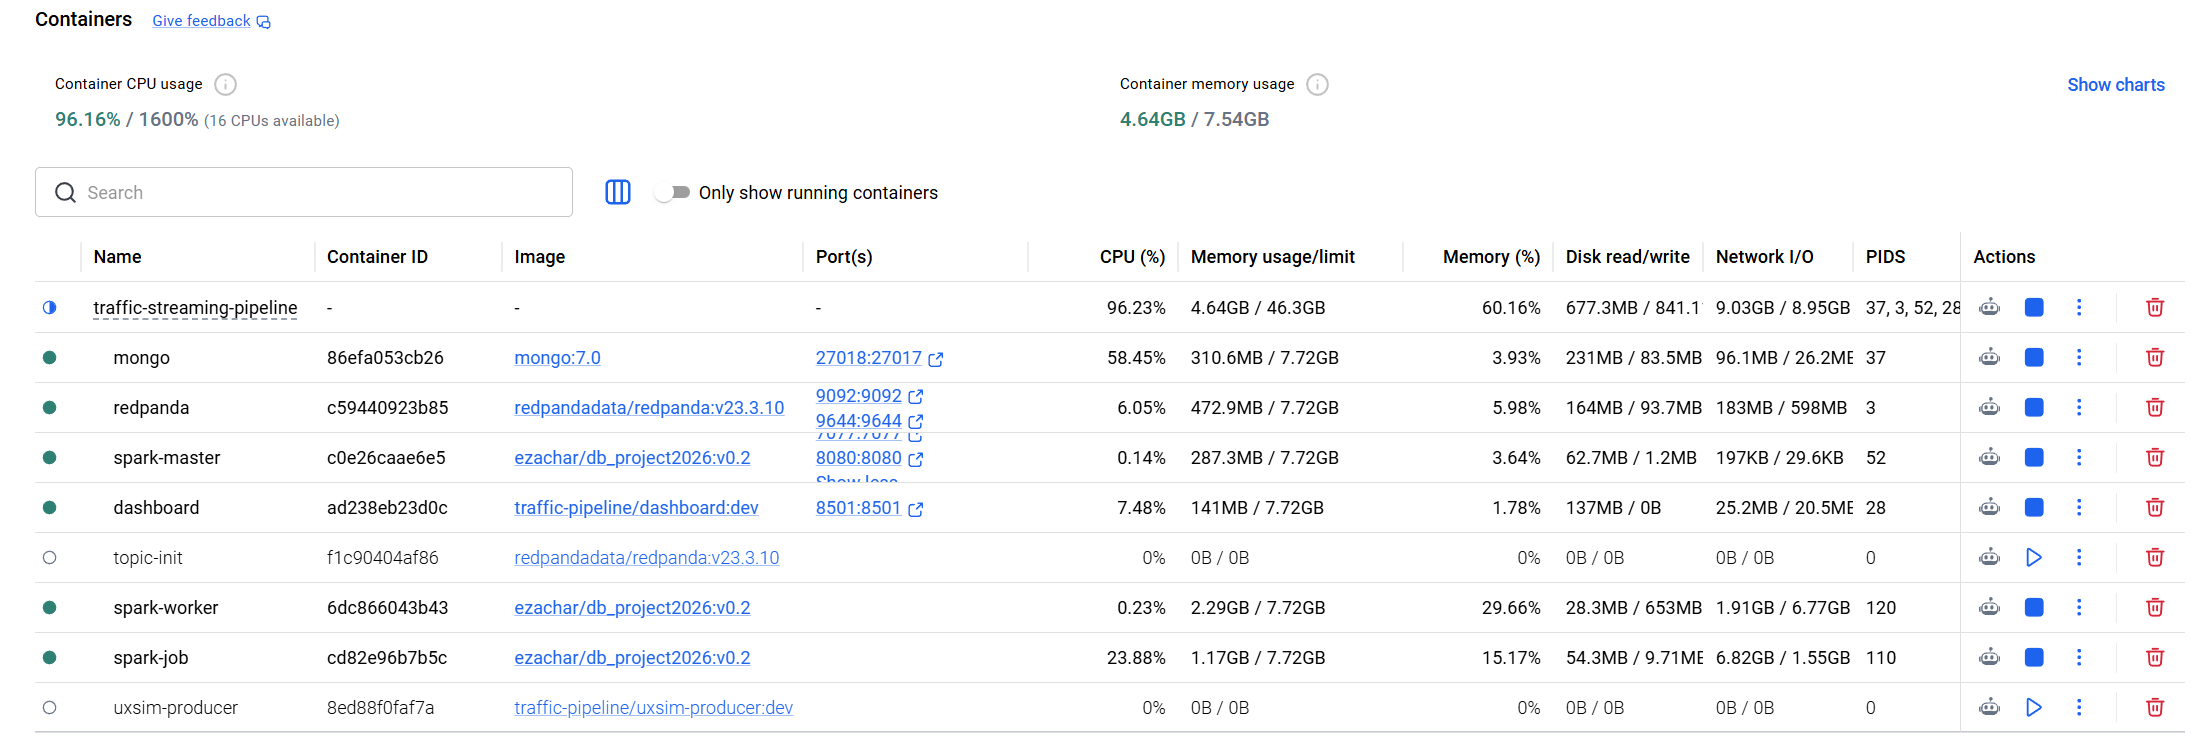
\includegraphics[width=\linewidth]{img/docker_desktop_stack.png}
   \caption{Docker Desktop, καρτέλα Containers με όλα τα services της στοίβας σε κατάσταση \emph{Running} (ισοδύναμο του Upstash dashboard).}
   \label{fig:docker}
\end{minipage}\hfill
\begin{minipage}[t]{0.48\textwidth}
   \centering
   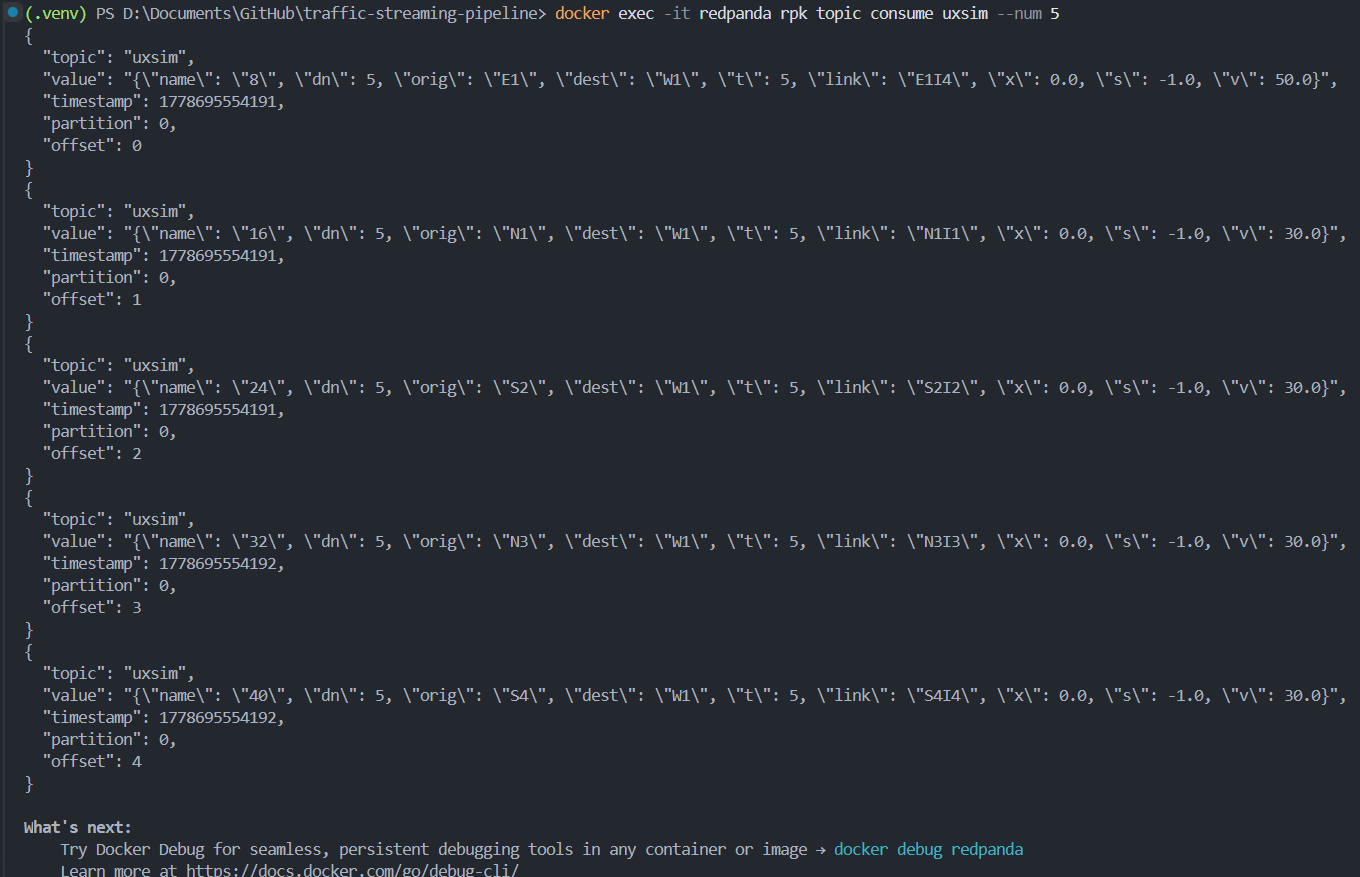
\includegraphics[width=\linewidth]{img/rpk_topic_consume.png}
   \caption{Έξοδος του \code{rpk topic consume} μέσα στο container Redpanda, με δείγμα μηνυμάτων JSON (ισοδύναμο του Upstash "Messages" tab).}
   \label{fig:rpk}
\end{minipage}
\end{figure}

\begin{figure}[!h]
\centering
\begin{minipage}[t]{0.48\textwidth}
   \centering
   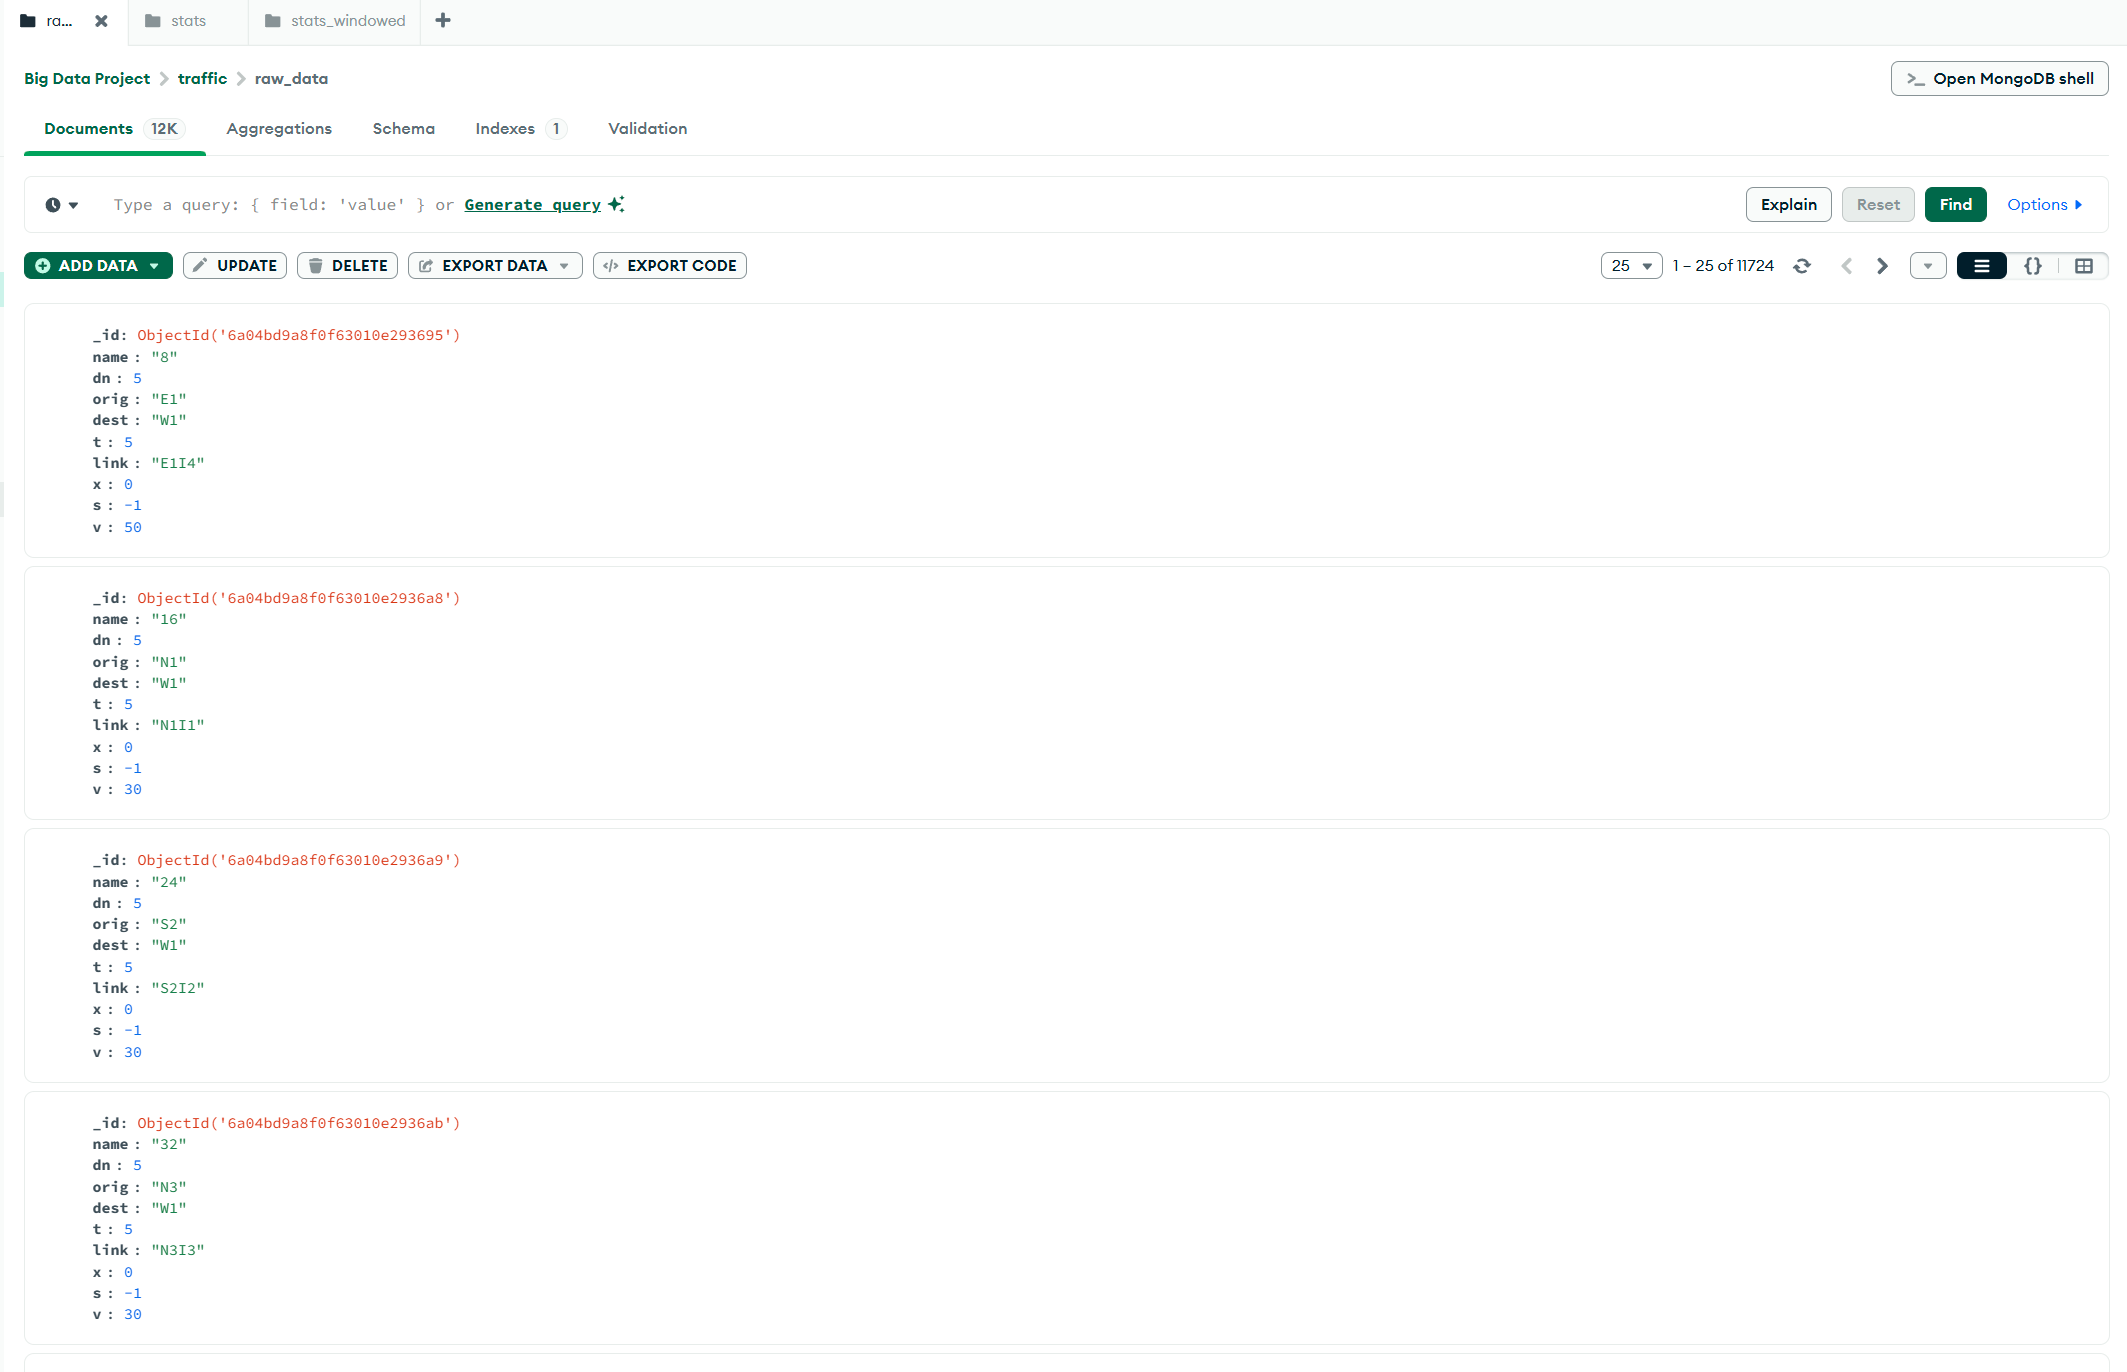
\includegraphics[width=\linewidth]{img/compass_collections.png}
   \caption{MongoDB Compass συνδεδεμένο στο \code{mongodb://localhost:27018}, με τις συλλογές \code{raw\_data}, \code{stats} και \code{stats\_windowed} της βάσης \code{traffic}.}
   \label{fig:compass}
\end{minipage}\hfill
\begin{minipage}[t]{0.48\textwidth}
   \centering
   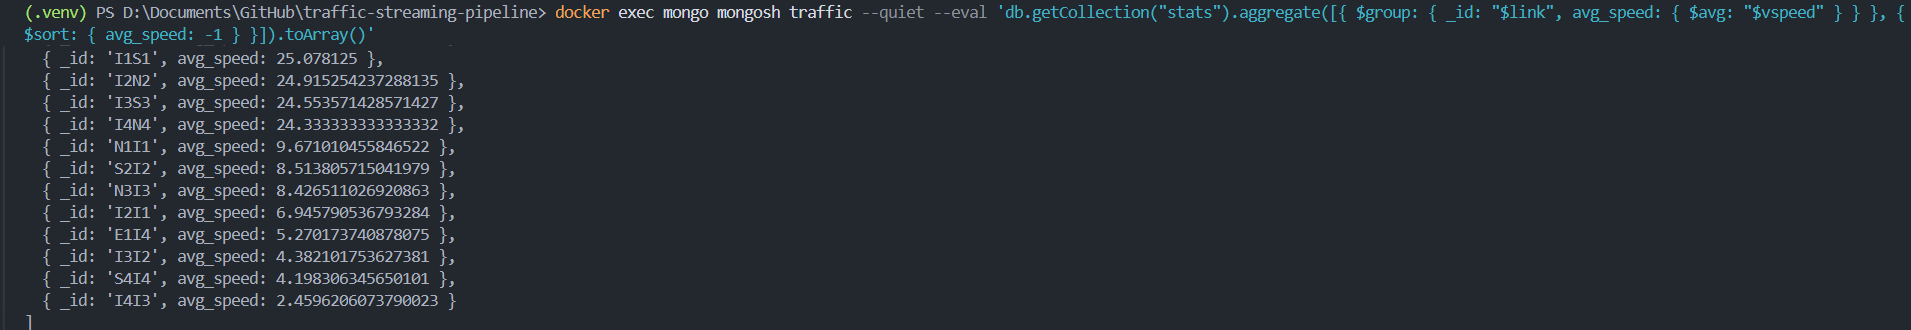
\includegraphics[width=\linewidth]{img/compass_aggregation.png}
   \caption{Η αναζητούμενη μέση ταχύτητα ανά link, εκτελεσμένη στο Aggregation tab του Compass (ισοδύναμα στο \code{mongosh}).}
   \label{fig:agg}
\end{minipage}
\end{figure}

\begin{figure}[!h]
\centering
\begin{minipage}[t]{0.48\textwidth}
   \centering
   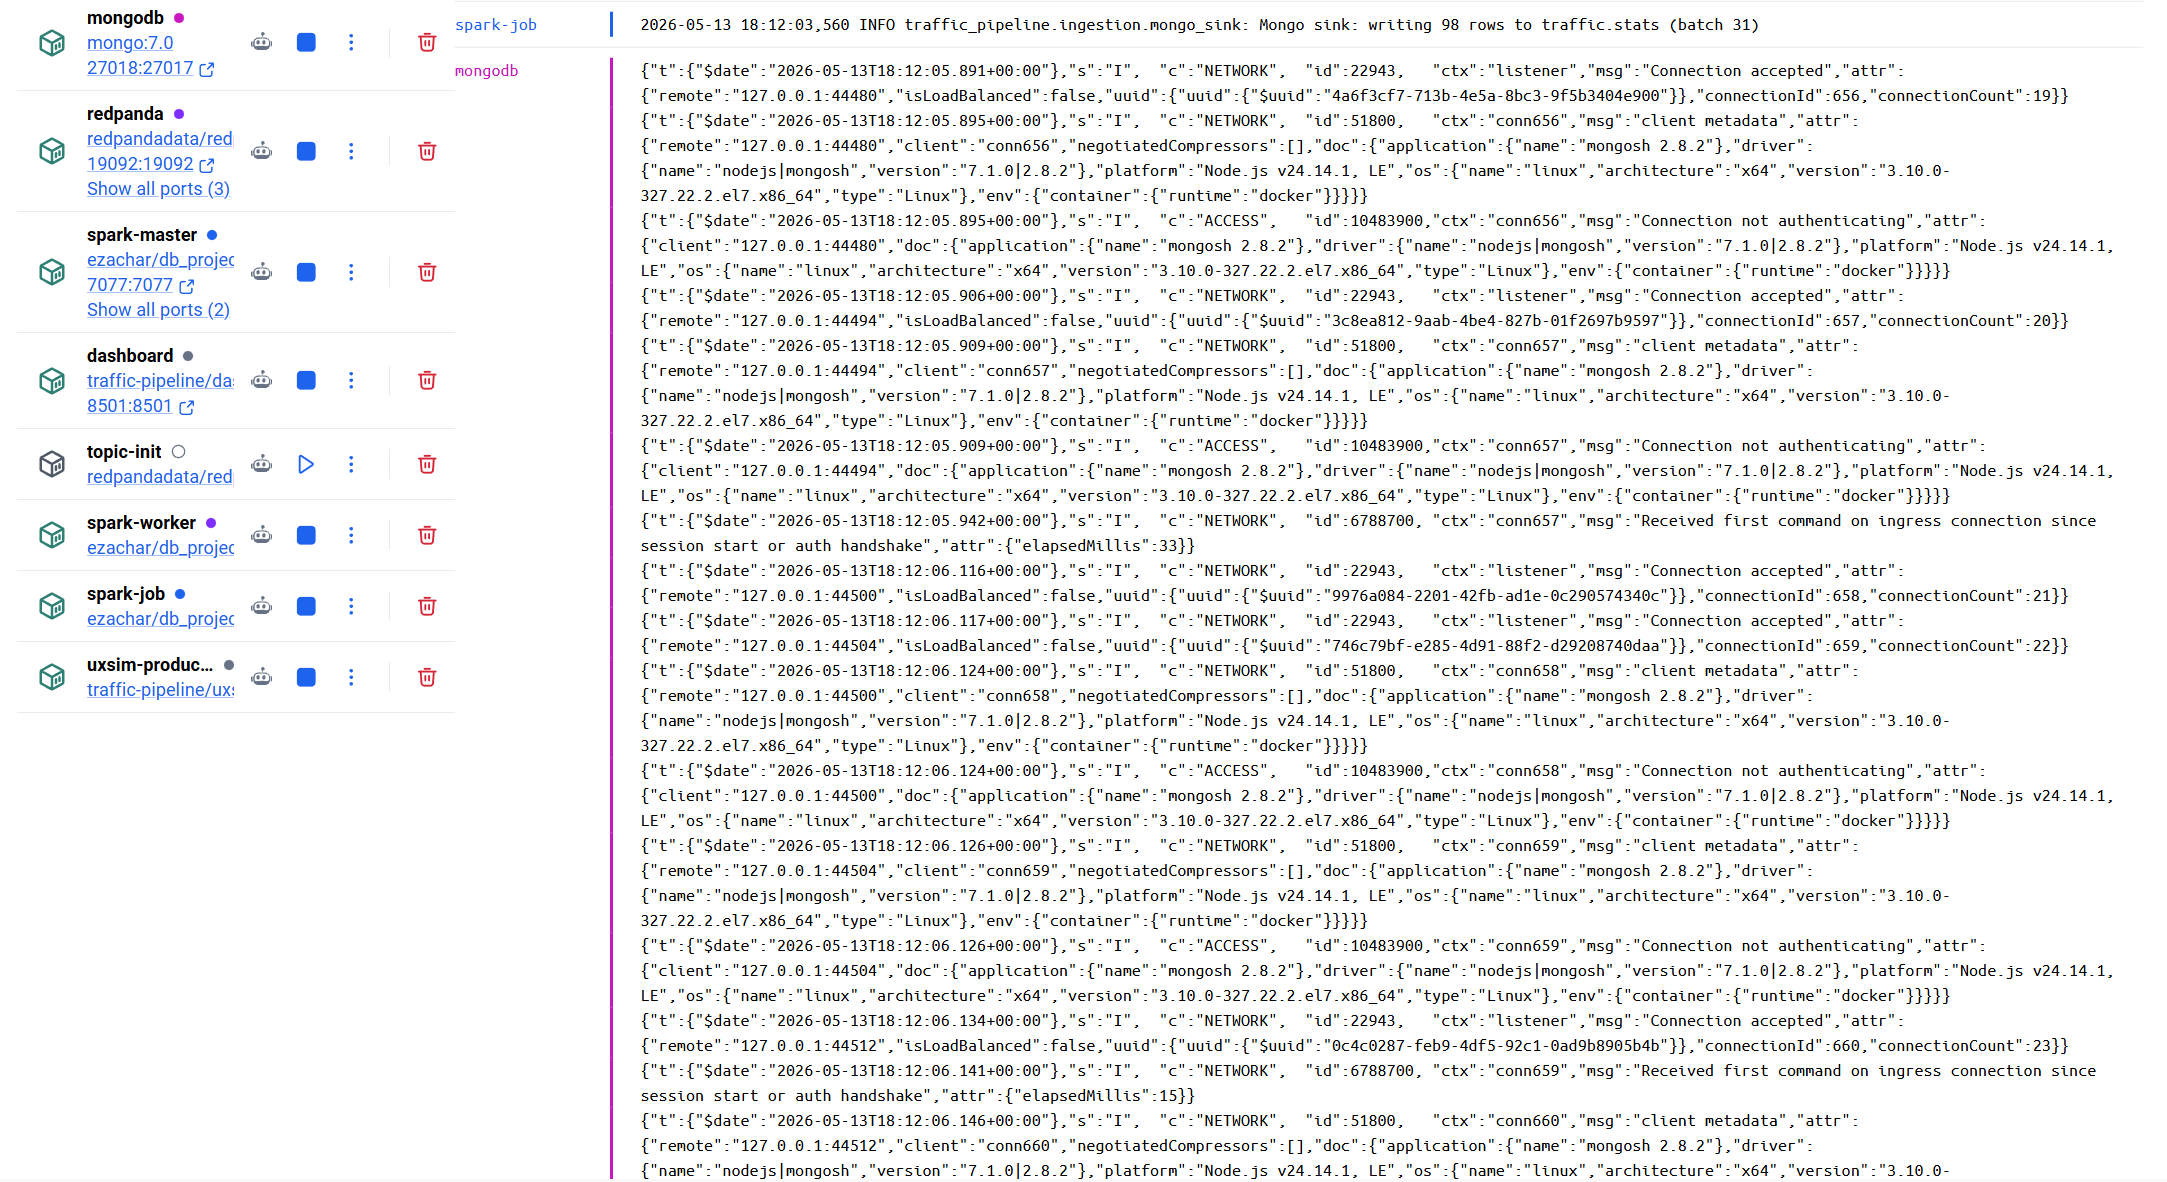
\includegraphics[width=\linewidth]{img/spark_console.png}
   \caption{\code{docker logs -f spark-job} με τα μηνύματα "Batch processed" του Structured Streaming (ενδεικτικά output του Spark console sink).}
   \label{fig:spark}
\end{minipage}\hfill
\begin{minipage}[t]{0.48\textwidth}
   \centering
   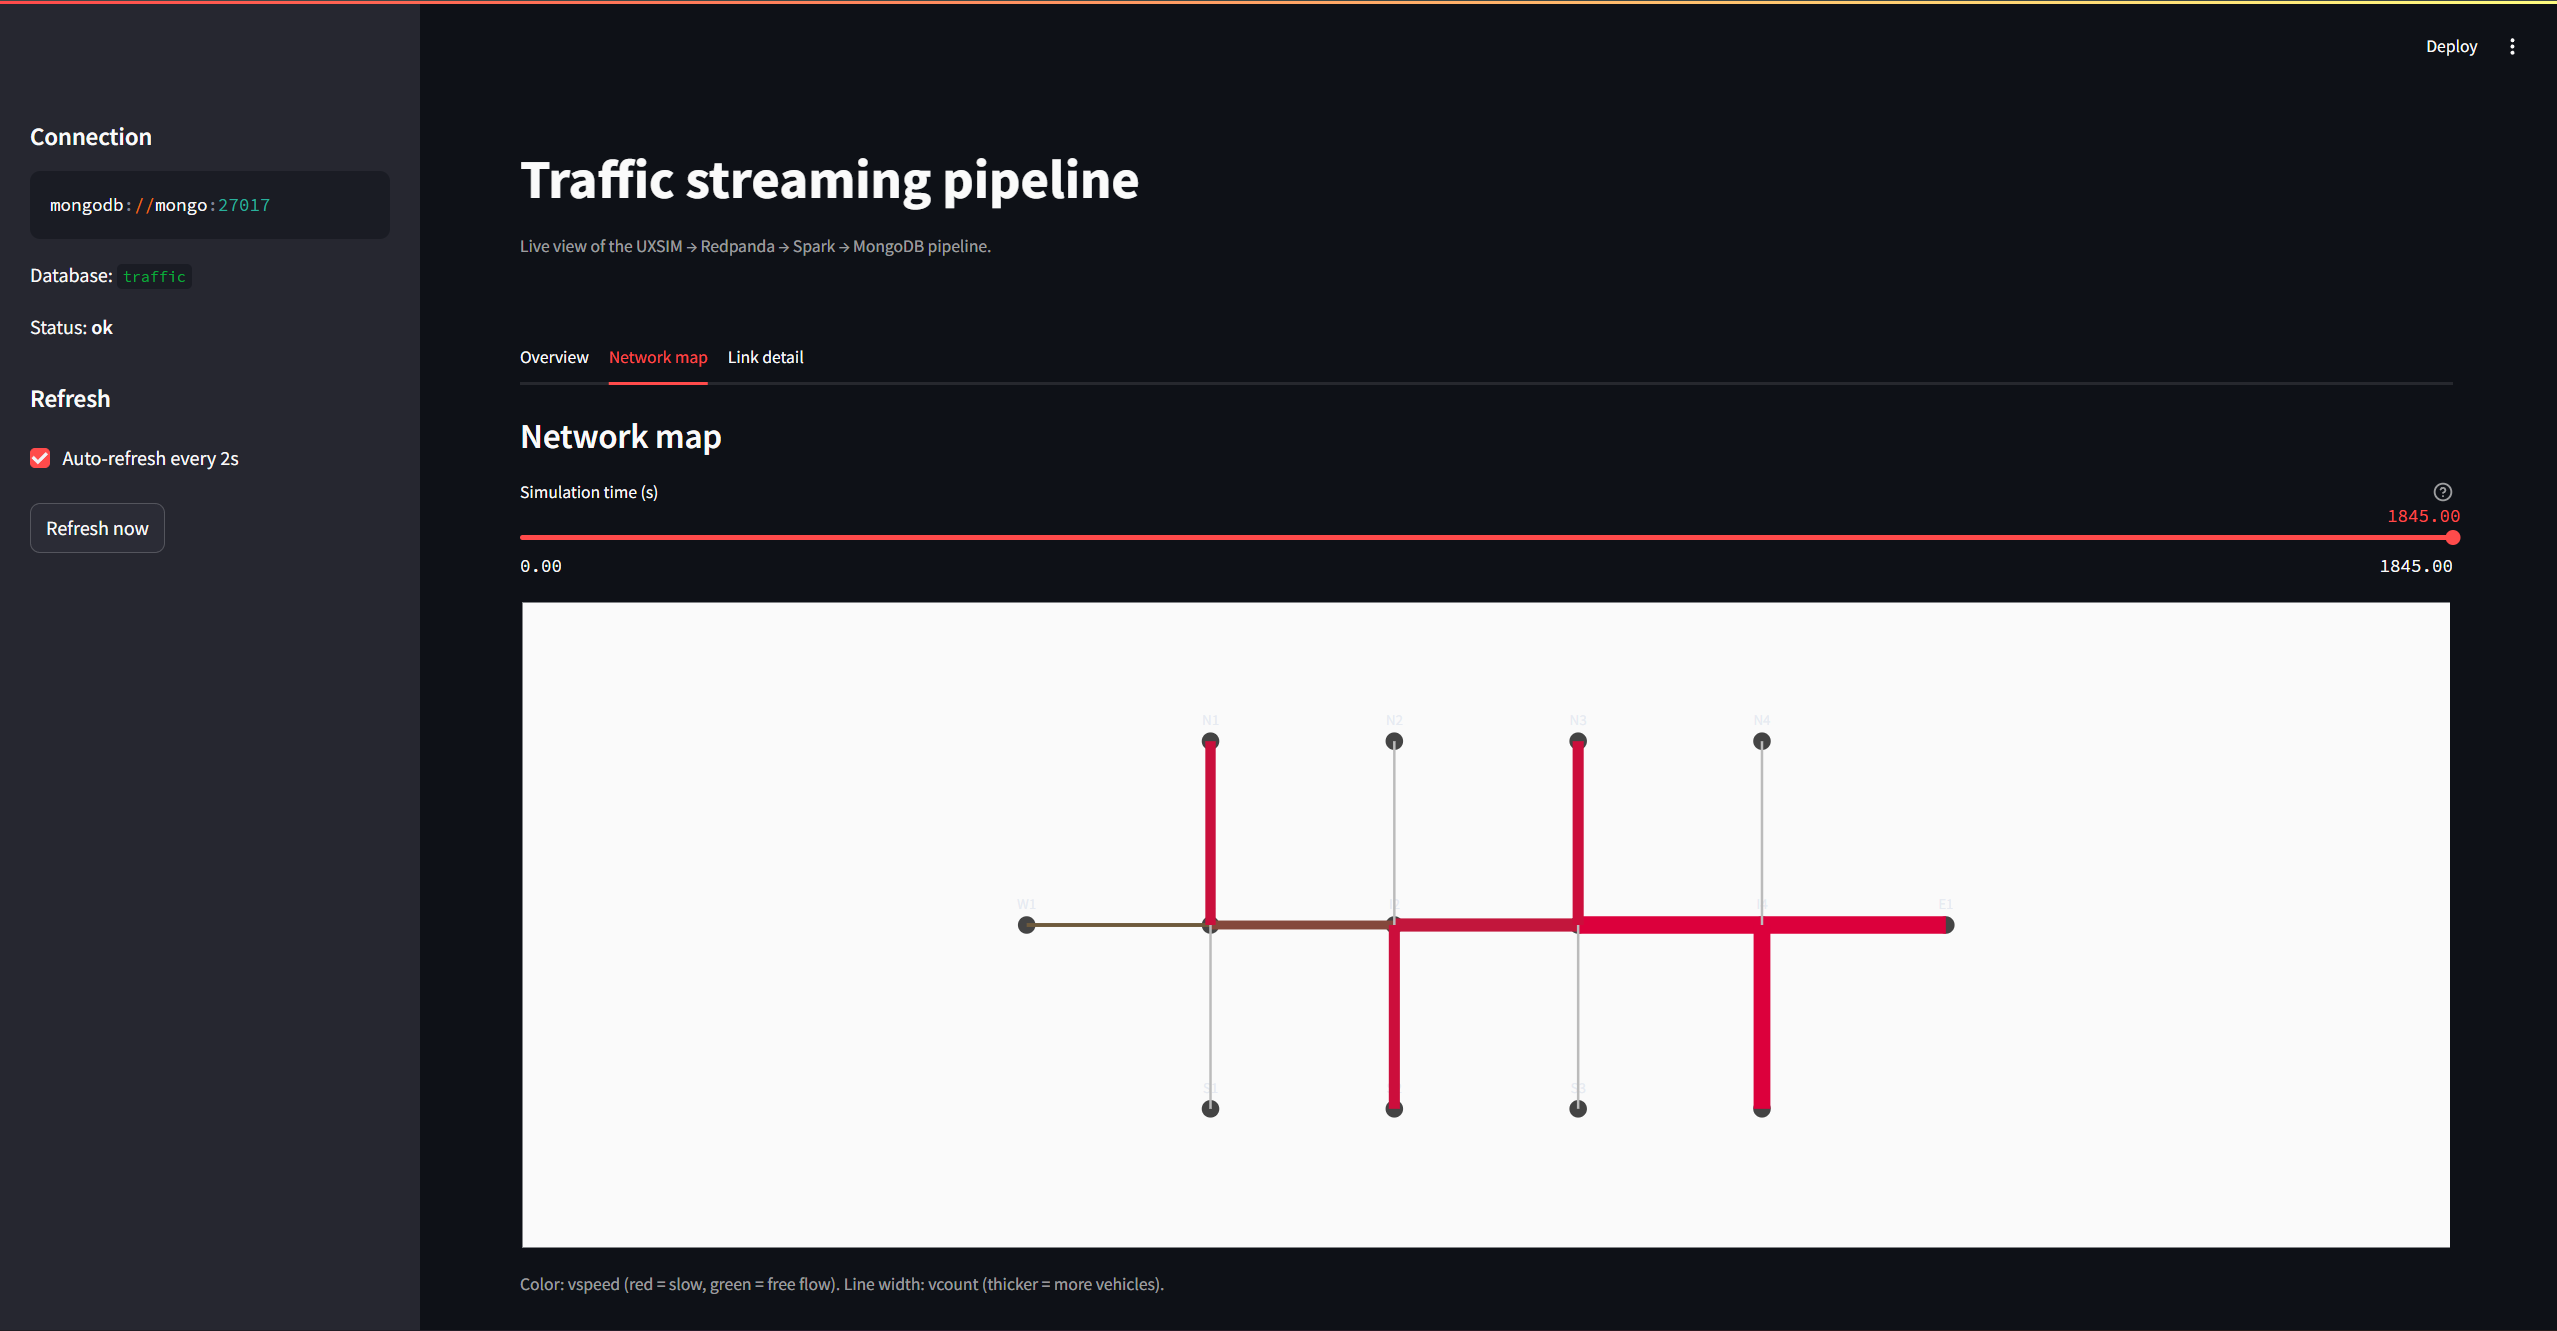
\includegraphics[width=\linewidth]{img/dashboard_map.png}
   \caption{Streamlit dashboard στο \code{http://localhost:8501}, καρτέλα \emph{Network map}, με χρωματισμό ακμών κατά \code{vspeed} (bonus παρουσίαση των δεδομένων).}
   \label{fig:dash}
\end{minipage}
\end{figure}

% ====================== §6 Problems ======================
\newpage
\section{Προβλήματα που Αντιμετωπίστηκαν}
\begin{itemize}
  \item \textbf{\code{kafka-python} 2.0.2 incompatibility με Python 3.12} (\code{ModuleNotFoundError: kafka.vendor.six.moves}). Λύση: pin σε \code{kafka-python-ng 2.2.3}, που είναι API-συμβατό fork.
  \item \textbf{Race condition στο πρώτο boot}, όπου ο producer ξεκινούσε πριν δημιουργηθεί το topic. Λύση: ξεχωριστό one-shot service \code{topic-init} και εξάρτηση μέσω \code{depends\_on: service\_completed\_successfully}.
  \item \textbf{Σύγκρουση πορτών MongoDB} στο host (τυπική τοπική εγκατάσταση στο 27017). Λύση: mapping σε \code{27018:27017} και ενημέρωση του \code{MONGO\_URI\_HOST}.
  \item \textbf{Windows + \code{spark.createDataFrame} sockets}, που πάγωναν σε integration tests. Λύση: αντικατάσταση των in-process Python rows με \code{spark.sql("VALUES ...")}, ώστε όλη η δουλειά να μένει στη JVM.
\end{itemize}

% ====================== §7 Conclusions ======================
\section{Συμπεράσματα και Μελλοντικές Επεκτάσεις}
Παραδίδεται ένα πλήρες, αναπαραγώγιμο pipeline που εκκινείται με μία εντολή Docker Compose, καλύπτει και τα τρία ερωτήματα της εκφώνησης και επεκτείνει το ζητούμενο με windowed aggregations, REST API και dashboard. Πιθανές μελλοντικές βελτιώσεις: idempotent upserts στη \code{stats} με σύνθετο \code{\_id = (t, link)} για ασφαλή επανεκτέλεση, alerting όταν η \code{vspeed} ενός link πέφτει κάτω από κατώφλι, μετακίνηση των checkpoints από \code{/tmp/} σε named volume για επιβίωση μετά από restart του cluster, και παραμετροποίηση της τοπολογίας του δικτύου από YAML αντί από Python literal.

% ====================== Bibliography ======================
% \bibliography{references}

\end{document}
